\documentclass[a4paper,11pt]{article}
\usepackage[a4paper,top=2.2cm,bottom=2.5cm,left=2cm,right=2cm,headheight=14pt]{geometry}
\usepackage[T1]{fontenc}
\usepackage[utf8]{inputenc}
\usepackage{lmodern}
\renewcommand{\familydefault}{\sfdefault}
\usepackage{microtype}
\usepackage{lastpage}
\usepackage{fancyhdr}
\pagestyle{fancy}
\fancyhf{}
\fancyhead[C]{Page \thepage{} of \pageref{LastPage}}
\renewcommand{\headrulewidth}{0.4pt}
\usepackage{graphicx}
\usepackage{xcolor}
\usepackage[most]{tcolorbox}
\usepackage{enumitem}
\usepackage[hidelinks]{hyperref}

\setlength{\parskip}{0.25em plus 0.05em}
\setlength{\parindent}{0pt}

% Spoken-line box -- what the operator says aloud.
\newtcolorbox{spoken}{
  enhanced,
  colback=blue!4,
  colframe=blue!50!black,
  boxrule=0pt,
  leftrule=2.5pt,
  arc=0pt,
  outer arc=0pt,
  left=7pt, right=7pt, top=3pt, bottom=3pt,
  fontupper=\itshape,
}

% Q&A: short B1 answer (default).
\newtcolorbox{shortans}{
  enhanced,
  colback=green!5,
  colframe=green!50!black,
  boxrule=0pt,
  leftrule=2.5pt,
  arc=0pt,
  outer arc=0pt,
  left=7pt, right=7pt, top=2pt, bottom=2pt,
  before skip=2pt, after skip=2pt,
}

% Q&A: deeper follow-up.
\newtcolorbox{deepans}{
  enhanced,
  colback=gray!8,
  colframe=gray!60,
  boxrule=0pt,
  leftrule=2.5pt,
  arc=0pt,
  outer arc=0pt,
  left=7pt, right=7pt, top=2pt, bottom=2pt,
  before skip=2pt, after skip=4pt,
}

\title{TartuBid Poster Session\\\large Speaking Guide for the Operator}
\author{Team: Anup Kumar \textbullet{} Md Mumin Ul Bari \textbullet{} Sten (Qun-yan Li)}
\date{5 June 2026 \textbullet{} 12:15--14:00\\Delta building, 2nd-floor lobby}

\begin{document}
\maketitle
\thispagestyle{fancy}

\noindent
This guide is for the person standing at the poster. It contains
everything you need to deliver the pitch, walk visitors through the
poster, run the live Python demo, and answer the questions you are
most likely to be asked. Read it cover-to-cover once before the
session, then flip to whichever section you need during it.

\medskip
\noindent
\textbf{Two visual conventions used throughout:}

\begin{spoken}
A blue-bordered italic block is something you say aloud. Read it
in a natural voice; you don't have to follow the words exactly.
\end{spoken}

\noindent
Plain prose starting with a verb (``Point at\ldots'', ``Open the
terminal\ldots'') is a stage direction for you, not something you
say.

\medskip
\noindent
\textbf{If you remember nothing else:} smile, slow down, and when
you don't know an answer, say so. ``Let me get back to you'' is
always better than guessing.

\vspace{1em}
\tableofcontents
\newpage

% ---------------------------------------------------------------
\section{Pre-session checklist}

Do this 15 minutes before the session starts. Tick each item.

\subsection*{Laptop}
\begin{itemize}[leftmargin=*,nosep]
  \item Battery is at least 70\,\% full, or charger is plugged in
        and working.
  \item Wi-Fi is connected. (You may need it to look something up,
        but the demo does not need it.)
  \item Screen brightness is high enough to be readable from arm's
        length.
  \item Notifications, Slack, email, and any chat apps are muted.
  \item One terminal window is open at this path:
\begin{verbatim}
C:\MSc-Computer-Science\Semester-2\ds\poster-session\tartubid
\end{verbatim}
  \item Dry-run the demo once to confirm it works:
\begin{verbatim}
python demo.py
\end{verbatim}
  You should see four lines starting with \texttt{Naive},
  \texttt{NTP}, \texttt{Berkeley}, and \texttt{TrueTime}. If you
  do not, see Section~\ref{sec:wrong} (``If something goes
  wrong'').
  \item Clear the terminal (\texttt{cls}) so the screen is empty
        and ready for the first visitor.
\end{itemize}

\subsection*{Poster and paper}
\begin{itemize}[leftmargin=*,nosep]
  \item The A0 poster is mounted on the board, facing visitors.
  \item This speaking guide is printed and on a small table or
        clipboard within arm's reach --- not held in your hands
        the whole time.
  \item A small notepad and pen are on the table, for visitor
        emails (Q\&A fallback in Section~\ref{sec:wrong}).
  \item A few QR-code stickers or business cards pointing at the
        team's GitHub or the detailed write-up, if you have them.
\end{itemize}

\subsection*{Personal}
\begin{itemize}[leftmargin=*,nosep]
  \item Water bottle within reach.
  \item Phone on silent, in your pocket, used \emph{only} for
        time-keeping --- not for scrolling.
  \item You know which of the three teammates is doing which
        time-slot, so you can hand over cleanly.
\end{itemize}

\subsection*{One-minute warm-up}
Read the elevator pitch in Section~\ref{sec:pitch} aloud once,
quietly. This is the moment to find a natural rhythm for the
opening sentence --- once a visitor is standing in front of you,
it is too late to rehearse.

\newpage

% ---------------------------------------------------------------
\section{Elevator pitch}\label{sec:pitch}

When a visitor walks up and stops in front of the poster, smile,
make eye contact, and read this aloud. Aim for 30--40 seconds.

\begin{spoken}
Hi! This is \textbf{TartuBid} --- our group's online-auction
prototype. The question behind it: when two computers' clocks
disagree by a few milliseconds, who really wins a close-call
auction? We compare three ways to keep clocks in sync --- NTP,
Berkeley, and Google's TrueTime --- and show why we chose NTP
plus a small safety zone around each deadline. Want me to run
the demo?
\end{spoken}

\subsection*{Delivery tips}
\begin{itemize}[leftmargin=*,nosep]
  \item Slow down on the project name (``TartuBid'').
  \item Pause briefly after ``a few milliseconds''.
  \item End with the question. If they nod or say ``sure'', go to
        Section~\ref{sec:walkthrough} (Walkthrough) and offer the
        demo at the end.
  \item If they just say ``oh, nice'' and walk on, say ``thanks
        for stopping by!'' and reset for the next visitor.
  \item Don't read the pitch from the page. Glance at it once if
        you blank, then look back up.
\end{itemize}

\subsection*{Variations}

If the visitor looks like a hurried passer-by, drop the last
sentence (the demo offer) and end with ``\ldots safety zone
around each deadline''. Total time: 25 seconds.

If the visitor is clearly an expert (you recognise them as the
professor, a TA, or another team's leader), shorten the framing
and lead with the design choice:

\begin{spoken}
Hi! TartuBid --- our distributed online auction. We compare NTP,
Berkeley, and TrueTime, and we adopt NTP plus a TrueTime-style
50-millisecond uncertainty band at the closing window. Happy to
walk you through it.
\end{spoken}

\newpage

% ---------------------------------------------------------------
\section{Walkthrough}\label{sec:walkthrough}

Use this if the visitor stays after the pitch. The poster has six
blocks. Take them in this order:

\begin{enumerate}[leftmargin=*,nosep]
  \item \textbf{Introduction} (top-left).
  \item \textbf{System model} (middle-left).
  \item \textbf{Mechanisms} (bottom-left).
  \item \textbf{Comparison and our choice} (top-right).
  \item \textbf{Prototype evidence} (middle-right).
\end{enumerate}

\noindent
The References block (bottom-right) is for the academic record ---
you do not need to walk through it unless a visitor asks for
sources. Figure~\ref{fig:thumb} shows where each block sits so you
can find the right one without staring at the wall.

\begin{figure}[h]
  \centering
  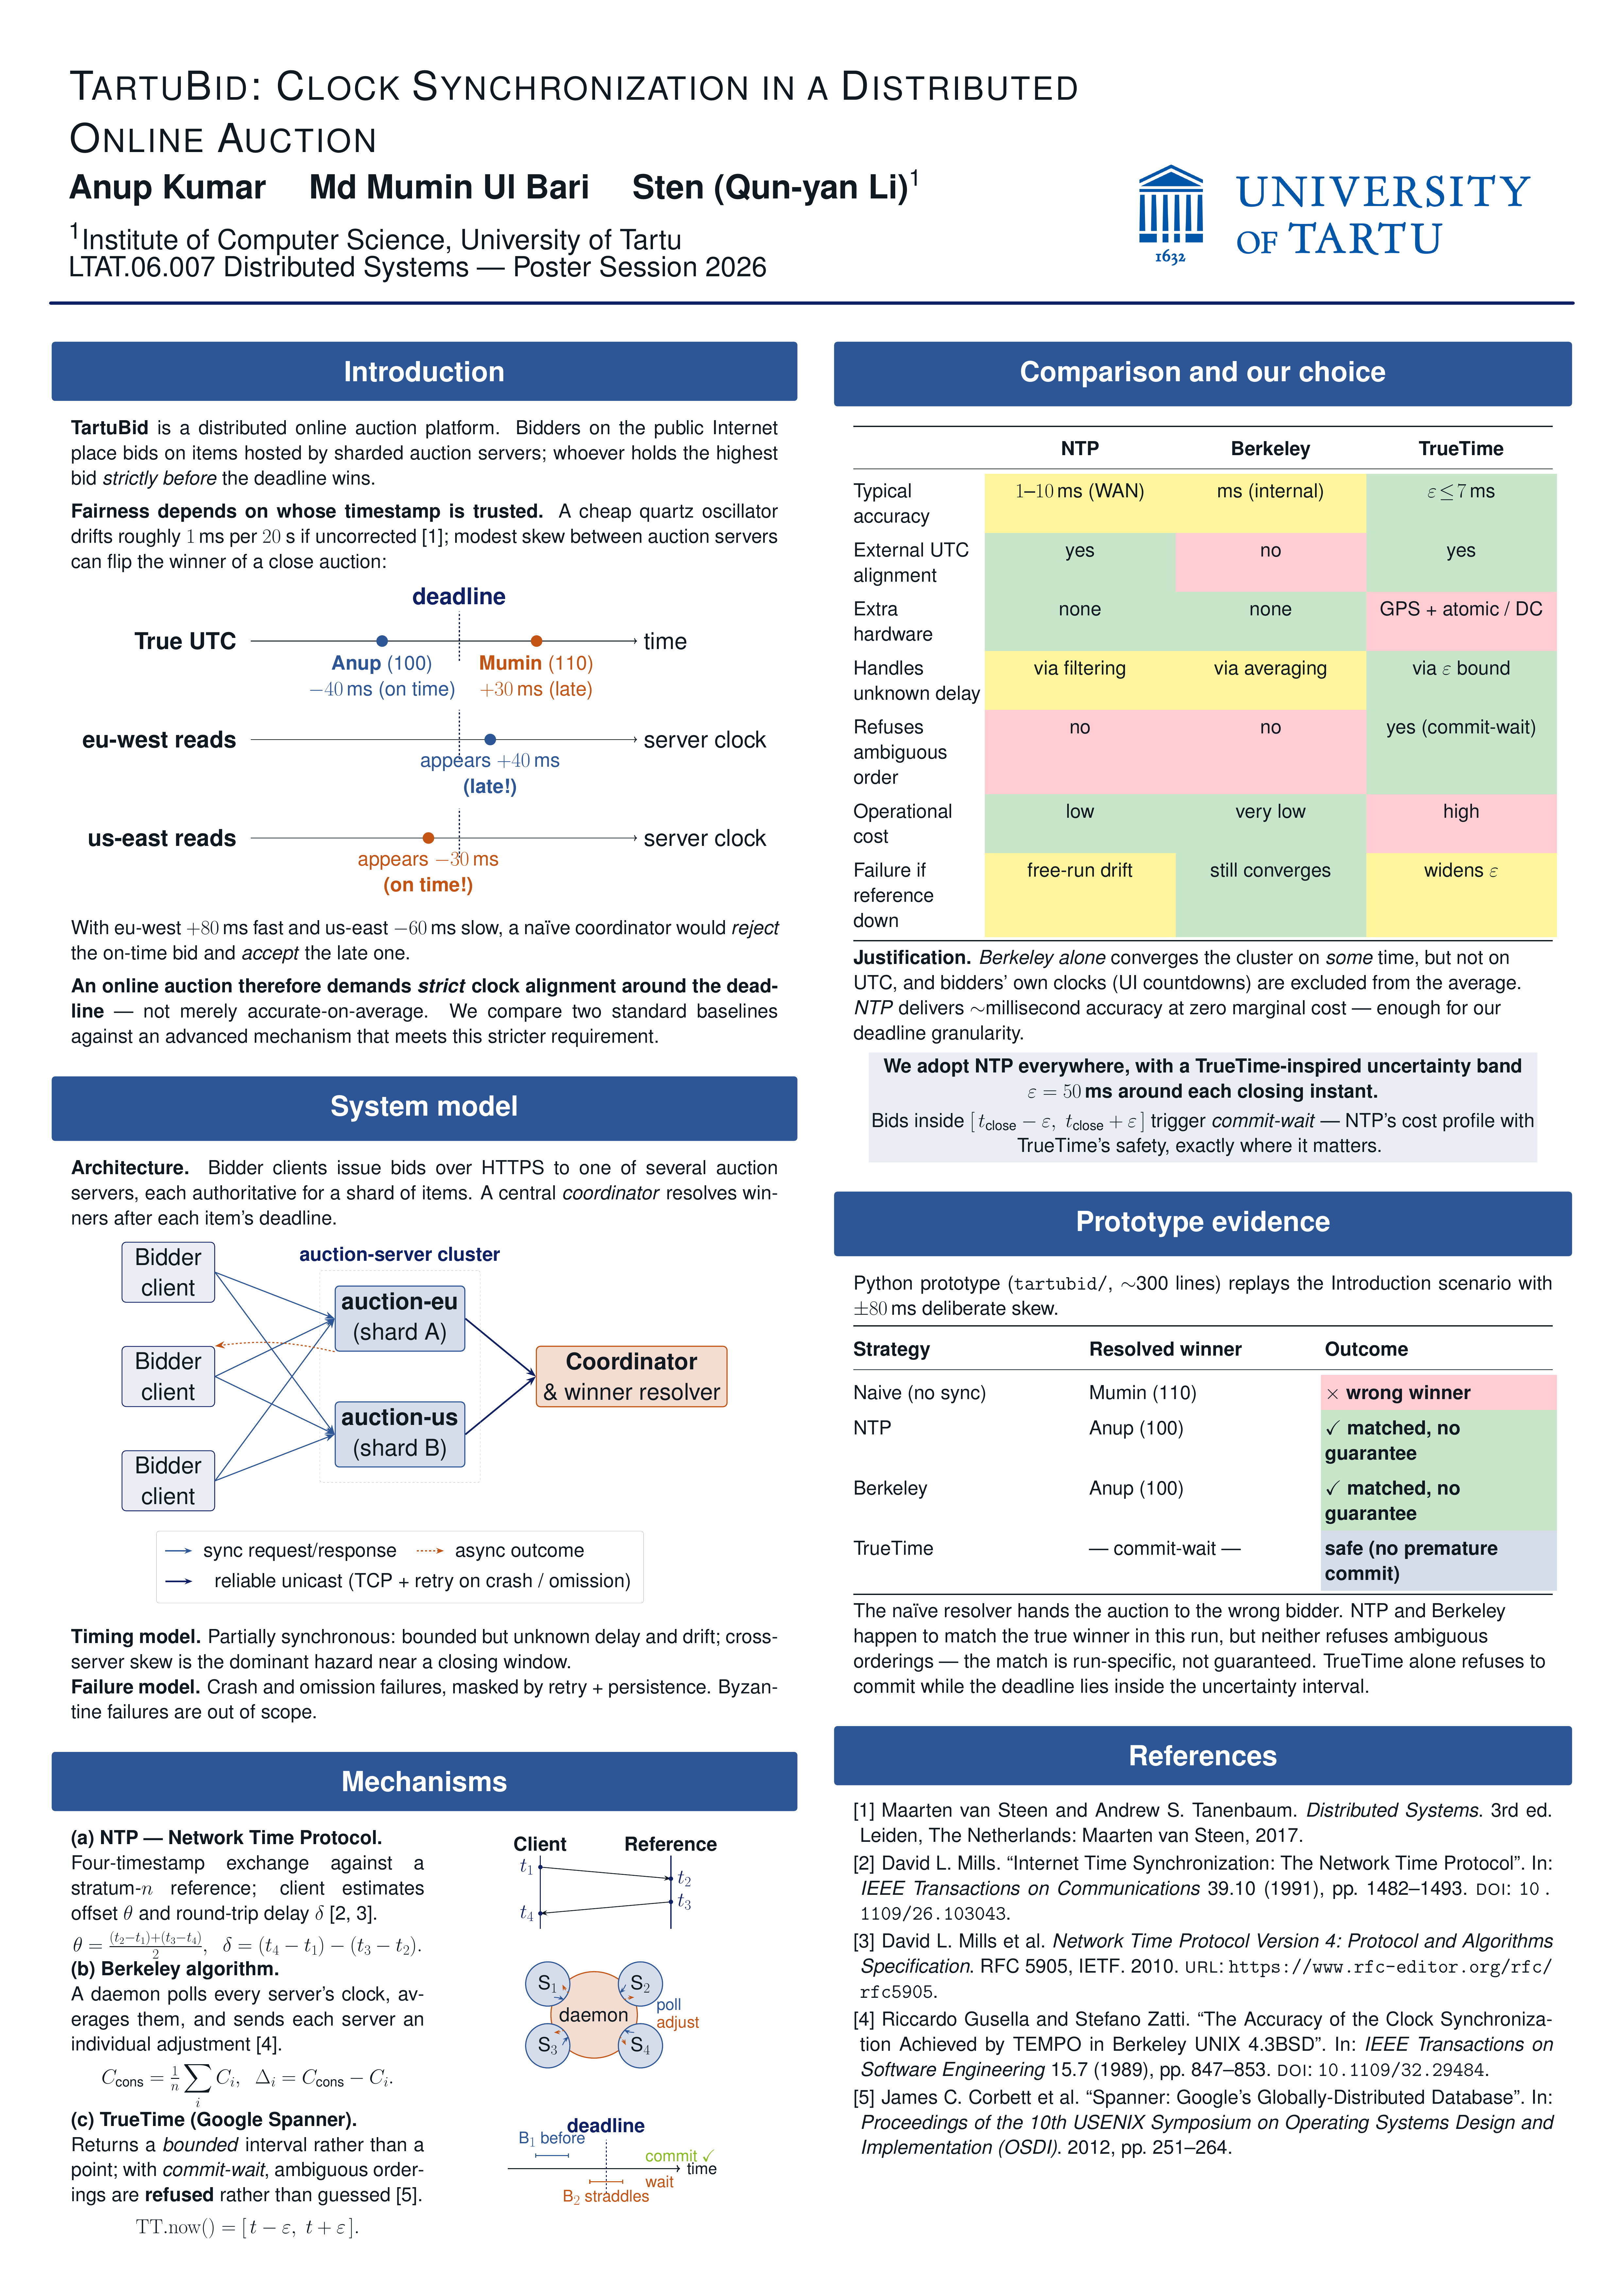
\includegraphics[width=0.55\textwidth]{assets/poster_thumbnail.png}
  \caption{Poster layout. Walk through it top-left, then down,
  then top-right, then down. The numbers in the order list above
  match the reading order.}
  \label{fig:thumb}
\end{figure}

The whole walkthrough takes 3--5 minutes. Don't rush. Pause after
each spoken block for the visitor to react.

\subsection{Stop 1 --- Introduction}

Point at the timeline picture with ``Anup'' and ``Mumin'' on it.

\begin{spoken}
This is the example we built the whole poster around. Anup bids
100 euros 40 milliseconds before the deadline --- that's on time.
Mumin bids 110 euros 30 milliseconds after the deadline --- that's
late. So Anup should win. But the two computers have clocks that
are off: one is 80 ms fast, the other is 60 ms slow. Once you add
the clock errors, Mumin's late bid \emph{looks} on time, and
Anup's on-time bid \emph{looks} late. A simple system would give
the auction to the wrong person.
\end{spoken}

\subsection{Stop 2 --- System model}

Point at the diagram with the bidder clients on the left and the
two auction servers on the right.

\begin{spoken}
Here's how the system is wired. People bid from their phones or
laptops. Their bids go to one of two regional servers --- say,
one in Europe and one in the US. A central piece called the
``coordinator'' decides the winner once the auction closes. The
solid arrows are normal requests. The dashed arrows are
notifications. The thick arrows go through TCP with retries, so
they survive small network glitches.
\end{spoken}

\subsection{Stop 3 --- Mechanisms}

Point at the three sub-boxes labelled (a), (b), (c).

\begin{spoken}
We picked three ways to handle the clock problem. NTP --- the
internet's standard way of keeping clocks aligned to global time.
Berkeley --- a method that averages the clocks of a small group of
computers. And TrueTime --- the system Google built for their
Spanner database. NTP and Berkeley give you a single ``best
guess'' of the time. TrueTime is different --- it tells you a
range, like ``the time is somewhere between this and this''. That
range is the key to its safety property.
\end{spoken}

\subsection{Stop 4 --- Comparison and our choice}

Point at the colour-coded table.

\begin{spoken}
This table compares the three methods. The colours show where
each one wins and loses. Look at the row ``Refuses ambiguous
order''. Only TrueTime says yes. That means only TrueTime knows
when to say ``I'm not sure, let me wait'' instead of guessing.
NTP is cheap and accurate enough. TrueTime is safe but expensive.
So our choice is the blue box at the bottom. We use NTP
everywhere, plus a small TrueTime-style safety band of 50
milliseconds around each deadline. Best of both worlds.
\end{spoken}

\subsection{Stop 5 --- Prototype evidence}

Point at the four-row results table.

\begin{spoken}
We actually built a small Python program to test this. Same
example as I showed at the start, with the same clock errors. The
naive method picks the wrong winner. NTP and Berkeley pick the
right one. TrueTime says ``commit-wait'' --- it refuses to declare
a winner while the deadline is inside its 50 ms uncertainty
window. It would wait a moment for the uncertainty to clear, then
resolve safely. If you want, I can run the program live --- it
takes about a second.
\end{spoken}

\textbf{If they say yes:} go to Section~\ref{sec:demo} (Live
demo).\\
\textbf{If they say no, or they look like they want to move on:}
thank them, and either let them go or offer to take one question
(go to Section~\ref{sec:qa}).

\newpage

% ---------------------------------------------------------------
\section{Live demo}\label{sec:demo}

The demo runs in about one second. Set up the screen \emph{before}
saying anything, then walk through the printed lines together with
the visitor.

\subsection*{Launching the demo}

\begin{enumerate}[leftmargin=*]
  \item Turn the laptop so the visitor can see the screen.
  \item In the terminal (already at the correct path from the
        pre-session checklist), type:
\begin{verbatim}
python demo.py
\end{verbatim}
        and press Enter.
  \item The whole output prints in well under a second.
\end{enumerate}

\subsection*{What the output looks like}

\begin{verbatim}
TartuBid -- clock-sync strategy comparison
------------------------------------------------------------
True deadline (UTC) : 1000000.000
Server skew         : {'eu-west': 0.08, 'us-east': -0.06}
Bids as recorded    :
  - Anup   100.00 @ eu-west (local stamp 1000000.050)
  - Mumin  110.00 @ us-east (local stamp  999999.970)

Naive (no sync)        -> winner: Mumin @ 110.0 EUR (via us-east)
NTP                    -> winner: Anup  @ 100.0 EUR (via eu-west)
Berkeley               -> winner: Anup  @ 100.0 EUR (via eu-west)
TrueTime               -> NO COMMIT  (commit-wait required:
                          2 bid(s) inside +/-50.0 ms uncertainty
                          window around deadline)
\end{verbatim}

\textbf{Note on the funny character.} On some Windows terminals
the ``$\pm$'' symbol (plus-minus) shows up as ``\texttt{?}'' or a
small box. That's only a font issue --- the program is fine. Just
read it as ``plus-minus 50 milliseconds''.

\subsection*{What to say while pointing at the screen}

Point at the four ``\texttt{->}'' lines, one at a time, as you
read.

\begin{spoken}
Top line: with no clock correction at all, the program picks
Mumin --- the wrong winner. Just like the poster shows.

Next two lines: NTP and Berkeley both correct the timestamps and
pick Anup --- the right winner.

Bottom line: TrueTime says ``no commit''. It noticed that both
bids fall inside the 50-millisecond uncertainty window around the
deadline, so it refuses to pick a winner. In the real Spanner
system, it would wait a few hundred milliseconds for the
uncertainty to clear, then decide. Safer than guessing.
\end{spoken}

\subsection*{Closing the demo}

\begin{spoken}
And that's the whole point of our design --- we keep NTP's low
cost and we borrow TrueTime's safety, but only at the deadline
where it actually matters.
\end{spoken}

\subsection*{Re-running for the next visitor}

The demo is the same every time --- numbers are fixed in the
script. Just clear the terminal (\texttt{cls} on Windows, or
press Ctrl-L) so the screen is empty again. Don't worry about
``resetting'' anything --- the program does not write to disk and
holds no state between runs.

\newpage

% ---------------------------------------------------------------
\section{Q\&A}\label{sec:qa}

Questions are ranked from most-common-or-important (top) to
least-common (bottom). For each one, read the \textbf{Short
answer} first --- it is the B1 default and is enough for most
visitors. Use \textbf{If they want more detail} only if the
visitor asks a follow-up or you can tell they want depth (the
professor, a TA, or a student who keeps nodding and asking
``but why?'').

\subsection{Q1. ``What is this poster about?'' \textnormal{\small\itshape (basic)}}

\begin{shortans}
It's about online auctions and computer clocks. When two
computers' clocks don't agree, a close auction can go to the
wrong person. We compare three ways to fix that.
\end{shortans}

\begin{deepans}
\textbf{If they want more detail:} The project is called TartuBid.
It's a small distributed online-auction system we built for the
course. We use it as the setting for comparing three
clock-synchronisation methods: NTP, Berkeley, and TrueTime. Then
we explain which one we chose for the auction case and why.
\end{deepans}

\subsection{Q2. ``Why does clock synchronisation matter for an auction?'' \textnormal{\small\itshape (basic)}}

\begin{shortans}
The rule is simple: ``the highest bid before the deadline wins''.
If the clocks lie by even 100 milliseconds, the wrong bid can
look like the right one. The example on the poster shows exactly
that.
\end{shortans}

\begin{deepans}
\textbf{If they want more detail:} A cheap quartz clock drifts
about 1 millisecond every 20 seconds when nothing corrects it.
For a long auction that drift is invisible. But for two bids that
arrive within 100 milliseconds of the deadline, that small drift
is enough to flip the winner. The fairness of the whole system
hinges on whose timestamp the coordinator trusts.
\end{deepans}

\subsection{Q3. ``What is TrueTime?'' \textnormal{\small\itshape (clarifying)}}

\begin{shortans}
TrueTime is Google's special clock service. Instead of saying
``the time is exactly X'', it tells you a range. Like ``the time
is somewhere between X minus 5 ms and X plus 5 ms''. It's honest
about what it doesn't know.
\end{shortans}

\begin{deepans}
\textbf{If they want more detail:} Google built TrueTime for their
Spanner database. They put GPS receivers and atomic clocks in
every data centre. The API returns an interval
$[t - \varepsilon, t + \varepsilon]$, where $\varepsilon$ is
usually 1--7 milliseconds. This lets Spanner do something called
\emph{commit-wait}: an operation doesn't commit until the whole
interval has moved past its assigned timestamp. After that, any
later operation in real time is guaranteed to get a later
timestamp.
\end{deepans}

\subsection{Q4. ``How does NTP work, in one minute?'' \textnormal{\small\itshape (clarifying)}}

\begin{shortans}
NTP keeps your computer's clock close to global time. Your
computer asks a time server ``what time is it?'', records the
round-trip, and then adjusts its own clock. It does that many
times and picks the best sample.
\end{shortans}

\begin{deepans}
\textbf{If they want more detail:} NTP exchanges four timestamps
with a reference server --- when the client sent the request, when
the server received it, when the server sent the reply, and when
the client received it. From those four numbers it computes the
network delay and the clock offset. It samples this many times,
keeps the eight most recent, and uses the one with the smallest
delay (because the least-delayed sample suffers the least
asymmetric-path bias). Over the public internet that gives you
about 10 ms accuracy.
\end{deepans}

\subsection{Q5. ``What's the Berkeley algorithm?'' \textnormal{\small\itshape (clarifying)}}

\begin{shortans}
A central computer asks every other computer in the group for its
clock. It averages the answers and tells each one to adjust to the
average. The whole group ends up agreeing on a time, but not on
the real global time.
\end{shortans}

\begin{deepans}
\textbf{If they want more detail:} The algorithm dates to 1980s
BSD Unix. One machine acts as the ``time daemon''. It polls all
machines for their clocks, drops obvious outliers, averages the
rest with its own clock, and sends each machine an individual
correction. Good for an isolated cluster --- you don't need any
external reference. But the cluster's consensus can quietly drift
away from real UTC, and you can't trust the resulting time as a
meaningful real-world date.
\end{deepans}

\subsection{Q6. ``What does `distributed' mean here?'' \textnormal{\small\itshape (basic)}}

\begin{shortans}
``Distributed'' means the system is made of many separate
computers that work together over a network. Each one has its own
memory, its own clock, and can fail on its own. That's why
coordination, like agreeing on the time, is hard.
\end{shortans}

\begin{deepans}
\textbf{If they want more detail:} In our system there are at
least three roles: the bidder's device, the regional auction
servers, and the coordinator. They don't share memory and they
don't share a clock. Anything they want to agree on --- like ``did
this bid arrive before the deadline?'' --- they have to negotiate
over the network. The whole distributed-systems course is about
that kind of negotiation under realistic failures.
\end{deepans}

\subsection{Q7. ``What is commit-wait?'' \textnormal{\small\itshape (clarifying)}}

\begin{shortans}
Commit-wait means ``don't decide yet, wait until you're sure''.
If a bid arrives in the uncertain window around the deadline, the
system waits. It waits for the uncertainty to pass, then decides
safely. It costs a bit of time but removes the risk of a wrong
call.
\end{shortans}

\begin{deepans}
\textbf{If they want more detail:} It's a pattern from Google's
Spanner. Each operation gets a timestamp $s$, and the system
holds the commit until \texttt{TT.now().earliest > s} --- until
the entire uncertainty interval has moved past $s$. After that,
any operation that happens later in real time is guaranteed to
get a later timestamp. We apply the same idea only at the auction
deadline: bids inside
$[t_\mathrm{close} - \varepsilon, t_\mathrm{close} + \varepsilon]$
are held, then resolved once $\varepsilon$ has drained.
\end{deepans}

\subsection{Q8. ``Why \texorpdfstring{$\varepsilon$}{epsilon} = 50 ms? How did you choose that?'' \textnormal{\small\itshape (probing)}}

\begin{shortans}
50 milliseconds is a balance. It's well above the noise we
usually see in NTP (around 10 ms), so we don't trigger commit-wait
on normal bids. And it's well under what a person can feel
(around 250 ms), so the small extra delay doesn't bother users.
\end{shortans}

\begin{deepans}
\textbf{If they want more detail:} We picked 50 ms as a defensible
default for the prototype, not a measured value. In a real
deployment we would measure the actual NTP jitter between our
cloud regions and set $\varepsilon$ from that data. The system
could also widen $\varepsilon$ dynamically when the network gets
worse --- Spanner does the same thing, growing $\varepsilon$ when
synchronisation falls behind.
\end{deepans}

\subsection{Q9. ``The table says NTP and Berkeley got the right winner but you call it `no guarantee'. What does that mean?'' \textnormal{\small\itshape (probing)}}

\begin{shortans}
In our test run, NTP and Berkeley happened to pick the right
person. But if the clock error had been a bit different, they
could have picked the wrong one. They don't know they might be
wrong. TrueTime is the only one that says ``I'm not sure'' when
it's not sure.
\end{shortans}

\begin{deepans}
\textbf{If they want more detail:} NTP and Berkeley return a
single best-guess time. If the bid is on the wrong side of the
deadline by a few microseconds, they will still confidently
declare a winner. Their correctness in our run is a property of
this specific scenario, not a guarantee. TrueTime returns an
interval and uses commit-wait, so it never declares a winner
while the deadline is inside the uncertainty. That's the safety
property our final design keeps, on top of NTP's cost profile.
\end{deepans}

\subsection{Q10. ``Why not just use Berkeley everywhere?'' \textnormal{\small\itshape (probing)}}

\begin{shortans}
Two reasons. First, Berkeley only aligns the servers, not the
bidders' own phones --- so the countdown the bidder sees can
disagree with the server. Second, Berkeley doesn't link to global
time, so the published deadline ``auction closes at 18:00'' has
no real-world meaning.
\end{shortans}

\begin{deepans}
\textbf{If they want more detail:} Berkeley converges the cluster
on some common time, which is just the average of the cluster's
clocks. It doesn't anchor to UTC, so the published deadline has
no canonical meaning to anyone outside the cluster. And clients
(phones, laptops) are not part of the cluster, so their UI
countdowns are off. NTP fixes both: it anchors to UTC and is
available everywhere at zero marginal cost, since every cloud VM
already runs an NTP daemon.
\end{deepans}

\subsection{Q11. ``Why pick those three protocols specifically?'' \textnormal{\small\itshape (probing)}}

\begin{shortans}
The assignment asked for three methods to compare --- at least
one from the course, and at least one researched on our own. NTP
and Berkeley were in the lectures. TrueTime is the one we
researched. They sit at three different points on the
cost-versus-safety scale.
\end{shortans}

\begin{deepans}
\textbf{If they want more detail:} NTP is the de facto standard
on the public internet and was covered in lecture 4. Berkeley is
the classic intra-cluster algorithm and was also covered.
TrueTime, from Google's Spanner paper in 2012, is not in the
lectures and gives a fundamentally different guarantee --- bounded
uncertainty plus commit-wait. The three together cover the design
space: external sync, internal sync, and uncertainty-honest sync.
\end{deepans}

\subsection{Q12. ``Who did what on the team?'' \textnormal{\small\itshape (meta)}}

\begin{shortans}
We were three people: Anup Kumar, Md Mumin Ul Bari, and Sten
(Qun-yan Li). We split the work four ways: literature review,
system model, Python prototype, and the poster itself. Everyone
touched everything.
\end{shortans}

\begin{deepans}
\textbf{If they want more detail:} Anup and Mumin focused on the
NTP and Berkeley literature and on the comparison table. Sten
built the Python prototype and the prototype-evidence block on the
poster. All three of us reviewed the poster drafts together. The
longer write-up in our \texttt{documentation.md} lists every
reference and every design decision in more depth.
\end{deepans}

\subsection{Q13. ``Why an auction, why this topic?'' \textnormal{\small\itshape (meta)}}

\begin{shortans}
An auction is the cleanest example we could think of where a few
milliseconds of clock error can change the outcome. It makes the
abstract topic --- clock synchronisation --- feel concrete and easy
to picture.
\end{shortans}

\begin{deepans}
\textbf{If they want more detail:} We were assigned the
clock-synchronisation topic randomly. From the application ideas
on the table, an online auction is unusually time-sensitive: the
winner depends on a strict before/after relation around one
single instant. That makes every clock-sync question visible in
the outcome. We also picked it because the architecture --- a
sharded backend with a central coordinator --- is the same as any
e-commerce stack, so the system-model block doesn't feel made-up.
\end{deepans}

\subsection{Q14. ``What happens if your NTP reference goes down during an auction?'' \textnormal{\small\itshape (failure-mode)}}

\begin{shortans}
Each server keeps running on its own local clock. The clock
drifts slowly --- about 1 ms every 20 seconds. For a short
outage, the safety band around the deadline still catches close
bids; the system just gets less certain. For a long outage, the
band would have to be widened.
\end{shortans}

\begin{deepans}
\textbf{If they want more detail:} NTP failure means the clocks
``free-run''. A modern quartz clock drifts at around 50 parts per
million --- a few milliseconds per minute. For a closing window of
a few seconds that's fine. We could also widen $\varepsilon$
dynamically as time since the last good sync increases, which is
what TrueTime does in its production form. To survive long
outages cleanly the next step would be Precision Time Protocol
over hardware-supported network cards, or a local atomic clock
--- both out of scope for our prototype.
\end{deepans}

\subsection{Q15. ``What if a bid arrives during commit-wait?'' \textnormal{\small\itshape (failure-mode)}}

\begin{shortans}
The system records it and treats it the same way as the bids that
triggered the wait. Once the uncertainty has passed, all of them
are resolved together. Nothing is lost.
\end{shortans}

\begin{deepans}
\textbf{If they want more detail:} A bid that lands while
commit-wait is in progress is just another bid inside the
uncertainty window. The coordinator holds the resolution until
the window has closed for the latest such bid. At that point it
has a stable set of bids that are definitely before the deadline,
and it picks the winner from those. The cost is at most a few
hundred milliseconds of decision latency --- Spanner accepts the
same trade-off for serialised transactions.
\end{deepans}

% ---------------------------------------------------------------
\section{Transitions and quiet moments}

\subsection*{Ending one conversation cleanly}

When a visitor seems ready to leave, end on a clear note.

\begin{spoken}
Thanks for stopping by! If you want the full write-up, it's in
our GitHub repository --- I can point you to it. Have a good rest
of the session.
\end{spoken}

If they ask for the repository link, point at the QR code or
write the URL on a sticky note from the table.

\subsection*{Greeting the next visitor}

Once the previous visitor has moved one step away, turn back to
the poster, look up, and make eye contact with anyone within a
metre. If they hesitate, offer:

\begin{spoken}
Hi! Want a quick tour?
\end{spoken}

Most people will either say yes (then run the pitch) or say
``just looking'' (then smile and let them read in peace).

\subsection*{Handing over to a teammate}

When your time-slot ends and a teammate takes over:

\begin{enumerate}[leftmargin=*,nosep]
  \item Finish the current visitor properly. Don't hand over
        mid-conversation.
  \item Brief the next operator on anything unusual that
        happened: an interesting question that you promised to
        follow up on, a known visitor coming back, the demo
        misbehaving.
  \item Hand over this printed guide and the notepad.
\end{enumerate}

\subsection*{When no one is around}

\begin{itemize}[leftmargin=*,nosep]
  \item Stand to the side of the poster, not directly in front of
        it --- you're blocking it for passers-by.
  \item Sip water. Stretch.
  \item Re-read Section~\ref{sec:qa} (Q\&A) to keep the answers
        fresh.
  \item Confirm the demo still runs. Re-run it once if it has
        been more than 20 minutes since the last time.
  \item Don't pull out your phone --- it makes you look unavailable
        and visitors will not approach.
\end{itemize}

% ---------------------------------------------------------------
\section{If something goes wrong}\label{sec:wrong}

\subsection*{The demo fails or prints nothing}

If \texttt{python demo.py} prints an error or nothing at all:

\begin{enumerate}[leftmargin=*,nosep]
  \item Stay calm. Don't apologise repeatedly --- one short
        ``looks like the demo isn't cooperating right now'' is
        enough.
  \item Say:
\end{enumerate}

\begin{spoken}
The demo is being grumpy --- but the same result is on the
poster. Let me walk you through the table here.
\end{spoken}

\begin{enumerate}[leftmargin=*,nosep,resume]
  \item Walk the visitor through the Prototype-evidence table on
        the poster (Stop~5 in Section~\ref{sec:walkthrough}).
        Same numbers, same conclusion --- the table on the poster
        \emph{is} the demo result.
  \item Once the visitor leaves, try to diagnose. In the
        terminal:
\begin{verbatim}
python --version
python -c "from clock_sync import Bid; print('ok')"
\end{verbatim}
        If \texttt{python --version} fails, the laptop's Python
        install is broken --- skip the demo for the rest of the
        session.\\
        If the import fails, you are not in the
        \texttt{tartubid} directory --- use \texttt{cd} to get
        there.
\end{enumerate}

\subsection*{A question you can't answer}

Don't guess. A confidently wrong answer is the worst outcome.

\begin{spoken}
That's a great question. I'd want to check the details before
giving you a wrong answer. Could I get your email and follow up
later?
\end{spoken}

Write the email on a sticky note. After the session, ask Anup or
Mumin, or look it up in \texttt{documentation.md} (the longer
expert-facing write-up in the same repository).

\subsection*{A visitor who doesn't speak much English}

Slow down. Use shorter sentences. Point at the poster more, talk
less. Lean on the diagrams and the numbers --- they are the same
in every language. If you share another language with the
visitor, switch.

\subsection*{The laptop dies or Wi-Fi drops}

The demo does not need Wi-Fi --- it's a local script. If the
laptop itself is dead and you can't recover it, fall back
permanently to the Prototype-evidence table on the poster. The
poster is the artefact; the demo is a bonus.

\subsection*{A hostile or aggressive question}

Stay polite. Don't argue. Acknowledge the point, then redirect.

\begin{spoken}
Interesting point --- I'd like to talk more about that after the
session, if you have time. Right now I should make sure the next
visitor gets a turn.
\end{spoken}

Then turn slightly towards the next visitor.

\subsection*{Two visitors arrive at once}

Pick the one who arrived first to start the pitch with, and
acknowledge the other briefly: \emph{``Hi! I'll be with you in a
minute --- feel free to read while you wait.''} Most second
visitors will have specific questions ready by the time you turn
to them.

% ---------------------------------------------------------------
\section{Appendix: glossary card}

A short reference for words you may hear from a visitor or might
need yourself. Skim it once before the session.

\begin{description}[leftmargin=*,style=nextline]
  \item[Clock skew] The difference between two computers' clocks
        at the same real-world moment.
  \item[Clock drift] The rate at which a clock gains or loses
        time as it runs. About 1 ms every 20 s for a cheap quartz
        oscillator.
  \item[NTP] Network Time Protocol. The standard way computers on
        the internet keep their clocks aligned to global time
        (UTC).
  \item[Stratum] A level in the NTP hierarchy. Stratum 0 is an
        authoritative time source (atomic clock, GPS). Stratum 1
        servers connect directly to one. Higher numbers are
        further away.
  \item[UTC] Coordinated Universal Time. The global time
        standard. ``Real time'' for the purposes of this poster.
  \item[Berkeley algorithm] A 1980s method where one machine
        averages the clocks of a group and tells each member how
        much to adjust.
  \item[TrueTime] Google's clock service. Returns an interval
        $[t - \varepsilon, t + \varepsilon]$ instead of a single
        time. Used by Google Spanner.
  \item[Spanner] Google's globally distributed database. Famous
        for using TrueTime to guarantee strict ordering of
        transactions across continents.
  \item[Commit-wait] The pattern of waiting until the uncertainty
        interval has passed before committing a result. Trades a
        small delay for a strong correctness guarantee.
  \item[Epsilon ($\varepsilon$)] The half-width of the
        uncertainty interval. We use $\varepsilon = 50$~ms in
        TartuBid.
  \item[Coordinator] In TartuBid, the central service that
        resolves the auction winner once the deadline has passed.
  \item[Shard] One of several pieces a system is split into, each
        holding part of the data. TartuBid's items are sharded
        across two auction servers (eu-west, us-east).
  \item[Partially synchronous] A timing model where message delay
        and clock drift are bounded but the bounds are not known
        in advance. This is the model we assume.
  \item[Byzantine failure] A failure where a component lies or
        behaves arbitrarily, instead of just crashing. We treat
        these as out of scope for the prototype.
  \item[PTP] Precision Time Protocol (IEEE 1588). A more accurate
        alternative to NTP, designed for local networks with
        hardware support. Mentioned as future work.
\end{description}

\medskip
\textbf{Cross-reference.} The expert-facing companion to this
guide is \texttt{documentation.md} at the root of the
\texttt{poster-session} repository. If a question goes deeper than
this guide, check there first.

\end{document}
